\documentclass[12pt]{article}
\usepackage{graphicx}
\usepackage{hyperref}
\usepackage{listings}
\usepackage{xcolor}

% Define colors for code listings
\definecolor{codegreen}{rgb}{0,0.6,0}
\definecolor{codegray}{rgb}{0.5,0.5,0.5}
\definecolor{codepurple}{rgb}{0.58,0,0.82}
\definecolor{backcolour}{rgb}{0.95,0.95,0.92}

% Configure code listing style
\lstdefinestyle{mystyle}{
    backgroundcolor=\color{backcolour},   
    commentstyle=\color{codegreen},
    keywordstyle=\color{magenta},
    numberstyle=\tiny\color{codegray},
    stringstyle=\color{codepurple},
    basicstyle=\ttfamily\footnotesize,
    breakatwhitespace=false,         
    breaklines=true,                 
    captionpos=b,                    
    keepspaces=true,                 
    numbers=left,                    
    numbersep=5pt,                  
    showspaces=false,                
    showstringspaces=false,
    showtabs=false,                  
    tabsize=2
}
\lstset{style=mystyle}

\title{Lab Assignment Instructions}
\author{Dr. Frank Xu}
\date{\today}

\begin{document}

\maketitle

\section*{Objective}
The objective of this lab assignment is to guide you through the process of executing commands and Python code as outlined in the provided PowerPoint (PPT) presentation. You will practice these commands and code snippets, capture screenshots of your work, and provide explanations for each step. Additionally, you will document any error messages encountered during the installation or execution process.

\section*{Instructions}
Each assignment must be written using the following guidelines:
\begin{itemize}
    \item Standard 8.5" x 11" page size
    \item 11 point or higher font for any text, source code, and text that is part of an image and screenshot.
\end{itemize}


\subsection*{Step 1: Access the Lab Instructions}
\begin{enumerate}
    \item Open the provided PowerPoint (PPT) file containing the lab instructions.  To access the lab instructions and resources, visit the following link:
          \begin{itemize}
              \item \href{https://github.com/frankwxu/digital-forensics-lab/tree/main/Basic_Computer_Skills_for_Forensics}{PPTs in GitHub Repository}.
          \end{itemize}
    \item Download lecture PPTs. The following image \ref{fig:lab-structure} demonstrates how to download PPTs:

          \begin{figure}[h!] % [h!] ensures the image is placed "here" if possible
              \centering % Center the image
              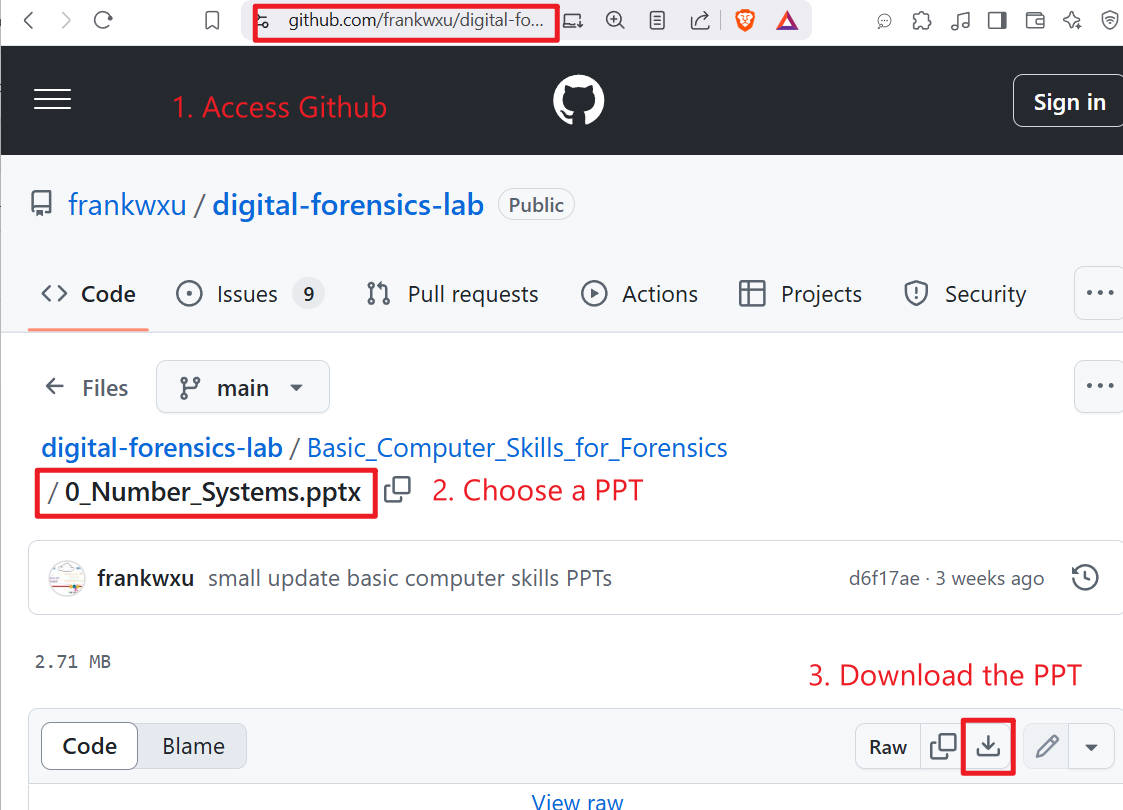
\includegraphics[width=1\textwidth]{images/download_ppt.jpg} % Replace with your image file name
              \caption{Steps to download PPTs} % Caption for the image
              \label{fig:lab-structure} % Label for referencing the image
          \end{figure}

    \item Review the slides thoroughly to understand the sequence of tasks.
\end{enumerate}

\subsection*{Step 2: Execute Commands and Python Code}
\begin{enumerate}
    \item Open your terminal or command prompt.
    \item Follow the commands listed in the PPT slides. For example:
          \begin{lstlisting}[language=bash]
# Example Command
ls -l
    \end{lstlisting}
    \item Execute the Python code provided in the slides. For example:
          \begin{lstlisting}[language=Python]
# Example Python Code
import numpy as np

arr = np.array([1, 2, 3, 4, 5])
print("Array:", arr)
    \end{lstlisting}
    \item Ensure that you test each command and code snippet in the correct order.
\end{enumerate}

\subsection*{Step 3: Capture Screenshots}
\begin{enumerate}
    \item After executing each command or Python script, please capture a screenshot of the output. Ensure to crop out any unrelated information, such as empty spaces or error messages, to focus on the relevant results.
    \item Include these screenshots in your submission document. The screenshot resolution must be similar or higher to the example shown below.
    \item Label each screenshot clearly with the corresponding task or step number.
\end{enumerate}

The example screenshot for the command \texttt{ls -l} is shown in Figure \ref{fig:lab-command}

\subsection*{Step 4: Explain Your Work}
\begin{enumerate}
    \item For each command or Python code snippet, write a brief explanation of what it does. The font size of descriptions must be at least 11 points or higher.
    \item For example:
          \begin{itemize}
              \item \textbf{Command:} \texttt{ls -l}

                    The \texttt{ls} command stands for ``list'' and is used to display the contents of a directory.

                    The \texttt{-l} option modifies the behavior of \texttt{ls} to display the contents in a \textbf{long listing format}, providing detailed information about each file or directory.


                    .
              \item \textbf{Python Code:} The code imports the NumPy library and creates an array, then prints it.
          \end{itemize}

    \item Screen capture software: Snipaste from https://www.snipaste.com/ or Snipping tool from Microsoft.


          \begin{figure}[h!] % [h!] ensures the image is placed "here" if possible
              \centering % Center the image
              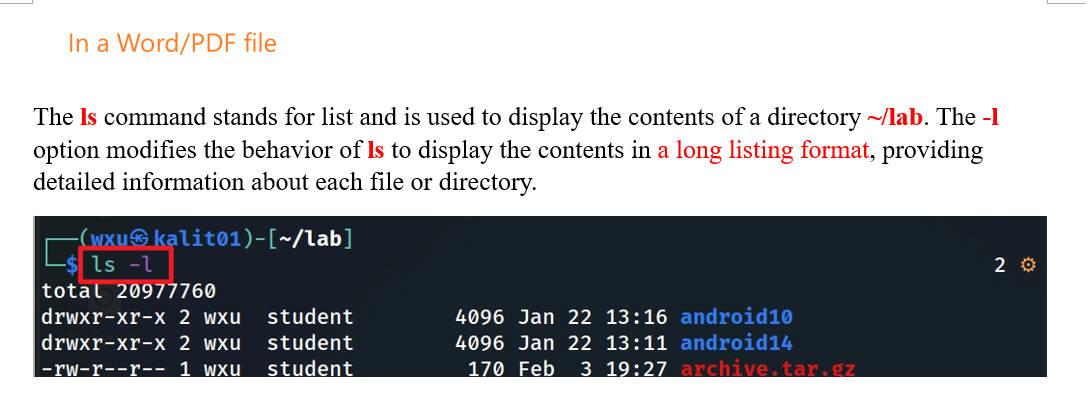
\includegraphics[width=1.1\textwidth]{images/command_explain.jpg} % Replace with your image file name
              \caption{An sample screenshot of the command \texttt{ls -l}} % Caption for the image
              \label{fig:lab-command} % Label for referencing the image
          \end{figure}



\end{enumerate}

\subsection*{Step 5: Handle Errors}
\begin{enumerate}
    \item If you encounter any error messages during the installation or execution process, record them.
    \item Take a screenshot of the error message and include it in your submission.
    \item Provide a brief description of the error and any troubleshooting steps you attempted.
    \item Note: Errors caused by differences in operating system versions or software versions will not impact your grade.
\end{enumerate}

\section*{Submission Guidelines}
\begin{itemize}
    \item Compile your screenshots, explanations, and error logs into a single PDF document.
    \item Use the following naming convention for your submission file: \\\texttt{LastName\_FirstName\_LabAssignment\_XXX.pdf}.
    \item Submit the PDF file via the course management system by the specified deadline (one week by default).
\end{itemize}

\section*{Grading Criteria}
Each lab is worth 10 points by default, unless otherwise specified during the class. A different problem-solving assignment will be provided if there is no hands-on practicing lab. Each problem-solving assignment is also worth 10 points.
\begin{itemize}
    \item Completion of all tasks: 50\%
    \item Accuracy of explanations: 30\%
    \item Quality of screenshots and documentation: 20\%
\end{itemize}

\section*{Additional Notes}
\begin{itemize}
    \item If you have any questions or need clarification, contact the instructor or teaching assistant.
    \item Ensure that you save your work frequently to avoid data loss.
\end{itemize}

\end{document}